% Advaitic robot learning assignment report (Overleaf-ready, pdfLaTeX).
% Sections marked \todo{} must be completed by the author before submission.
\documentclass[11pt,a4paper]{article}

\usepackage[margin=2.2cm]{geometry}
\usepackage[T1]{fontenc}
\usepackage{lmodern}
\usepackage{microtype}
\usepackage{booktabs}
\usepackage{amsmath}
\usepackage{xcolor}
\usepackage{listings}
\usepackage{pgfplots}
\pgfplotsset{compat=1.18}
\usepackage[colorlinks=true,linkcolor=blue!50!black,urlcolor=blue!50!black,citecolor=blue!50!black]{hyperref}

\newcommand{\todo}[1]{\noindent\textcolor{red!70!black}{\textbf{[TODO:} #1\textbf{]}}}
\lstset{basicstyle=\ttfamily\small,breaklines=true,columns=fullflexible,
  frame=single,framerule=0.3pt,rulecolor=\color{gray!60},backgroundcolor=\color{gray!5}}

\title{Plate Transfer with a Unitree G1:\\An ACT Imitation-Learning Baseline}
\author{\todo{Your name}}
\date{\todo{Date} \quad Commit: \texttt{\todo{SHA}}}

\begin{document}
\maketitle

\begin{abstract}
We train an Action Chunking with Transformers (ACT) policy on the 60 BiGym2
\texttt{move\_plate} human demonstrations to move a plate between two racks
with a Unitree G1 and Dex1-1 grippers, using only the three onboard cameras
and proprioception. The baseline does \emph{not} meet the 90\% criterion.
A 30-episode public run scored 27/30 (90\%), exactly at the threshold, but
larger 60-episode runs score 49/60 (81.7\%) on the public block and 48/60
(80.0\%) on a private validation block. Pooled over these two disjoint
blocks, the success rate is 97/120 (80.8\%). All failures are timeouts;
no episode ended in a fall.
\todo{Add one sentence on your improvement and its measured effect.}
\end{abstract}

%------------------------------------------------------------------------------
\section{Task and Interface}

The robot must move a plate from any of six source slots in rack~1 into any
slot of rack~2. Each rack varies by up to $\pm5$\,cm in $x/y$. Success requires the plate to be correctly
oriented, near a destination slot, touching rack~2, released by both
grippers and not supported by the table, held for one simulated second.
Falls, floor contact and the 1700-step (34\,s) budget end an episode as a
failure. Locomotion is provided by BiGym2's frozen Balance/Walk controller.

\paragraph{Observations.} \texttt{obs["rgb"]}: three $84\times84$ RGB
cameras (head, right wrist, left wrist); \texttt{obs["state"]}: 50-D
proprioception (arm and finger joints, pelvis pose and velocities, gripper
states). No simulator state, seed, slot or reward reaches the policy.

\paragraph{Actions.} 20-D, normalised to $[-1,1]$ with the public limits in
\texttt{action\_layout.json}: base forward/lateral velocity, pelvis height,
yaw rate, 14 arm joint targets and 2 gripper commands. The policy may return
a chunk of up to 50 actions per call.

%------------------------------------------------------------------------------
\section{Data}

BiGym2 provides 60 successful human teleoperation demonstrations
(37{,}645 control steps at 50\,Hz; 10.6--14.9\,s per episode). All 60 follow
the same strategy:
\begin{enumerate}
  \item reach the plate with the \emph{left} arm and close the left gripper
        (median step 230);
  \item lift the plate out of rack~1;
  \item side-step right by about 0.38\,m (range 0.30--0.41\,m) using base lateral
        velocity; pelvis height stays at 0.74\,m and yaw is not commanded;
  \item align and lower the plate into rack~2, then open the gripper
        (median step 569) and hold.
\end{enumerate}
The right gripper never closes. Source-slot coverage is uneven
(slots 1--6: 11, 6, 15, 8, 8, 12 demos). Demonstration seeds (18--147) are
disjoint from the public evaluation block (7{,}310{,}000+).

\paragraph{Two data-handling details.}
(i)~BiGym stores in row $t$ the observation \emph{and the action that
produced it}; row~0 is the reset row. We therefore pair observation $o_t$
with action row $t{+}1$.
(ii)~For base velocity (dims 0--1), the stored normalised \texttt{action}
field does not match the \texttt{action\_layout.json} normalisation of
\texttt{raw\_outer\_action} (differences up to 0.75). Dims 2--19 match. We
train on \texttt{raw\_outer\_action} in physical units and apply the
evaluator's normalisation at inference, so training and execution use the
same convention.

%------------------------------------------------------------------------------
\section{Method: ACT Baseline}

We re-implement ACT~\cite{zhao2023act} compactly in PyTorch (28.2M
parameters).

\paragraph{Encoder.} Each camera passes through an ImageNet-pretrained
ResNet-18 with frozen batch-norm, giving a $3\times3\times512$ feature map,
projected to $d=256$. This yields 27 image tokens with learned positional
and per-camera embeddings. A 4-layer transformer encoder processes these
together with a proprioception token and a latent token.

\paragraph{Decoder.} A 4-layer transformer decoder with 50 learned queries
outputs a 50-step (1\,s) chunk of raw actions, normalised by dataset mean
and standard deviation.

\paragraph{CVAE.} During training, a 4-layer transformer encodes the
ground-truth chunk and state into a 32-D latent $z$. The loss is
\begin{equation}
  \mathcal{L} = \lVert \hat a_{t:t+50} - a_{t:t+50}\rVert_1
  + \beta\, D_{\mathrm{KL}}\!\left(q(z\mid a, s)\,\Vert\,\mathcal{N}(0,I)\right),
  \qquad \beta = 10 .
\end{equation}
At inference $z=0$.

\paragraph{Training.} Batch 32, AdamW (lr $10^{-4}$, backbone $10^{-5}$,
weight decay $10^{-4}$), 1k-step warm-up then cosine decay, bf16 autocast,
gradient clipping at 10, and DrQ-style random-shift image augmentation
($\pm4$\,px). Chunks that run past an episode end repeat the final action,
which teaches the policy to hold still after release. We trained 200k steps
in 5.25\,h on one RTX~3050 Laptop GPU (4\,GB; 1.1\,GB used; 10.6
steps/s). Figure~\ref{fig:loss} shows the training loss.

\paragraph{Inference.} Two execution modes:
\emph{temporal ensembling}~\cite{zhao2023act}, which queries every step and
averages all overlapping predictions for the current step with weights
$w_i=e^{-0.01 i}$ ($i=0$ oldest; $k=0.01$ by default, varied in
Section~\ref{sec:ksweep}); and \emph{chunked}, which executes the first 10 actions of
each prediction. Inference takes about 4.5\,ms per step on the GPU (ensemble mode).
The policy runs in a separate Python environment through the evaluator's
\texttt{--policy-python} process boundary.

\begin{figure}[t]
\centering
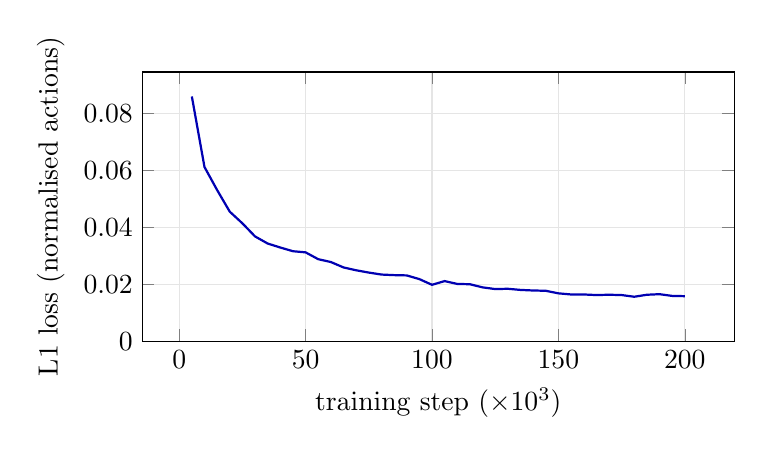
\begin{tikzpicture}
\begin{axis}[width=0.75\linewidth,height=5cm,xlabel={training step ($\times10^3$)},
  ylabel={L1 loss (normalised actions)},ymin=0,
  yticklabel style={/pgf/number format/fixed,/pgf/number format/precision=2},
  scaled y ticks=false,grid=major,grid style={gray!20}]
\addplot[thick,blue!70!black] coordinates {
(5,0.0860) (10,0.0612) (15,0.0531) (20,0.0455) (25,0.0414) (30,0.0368) (35,0.0343)
(40,0.0329) (45,0.0316) (50,0.0312) (55,0.0288) (60,0.0278) (65,0.0259) (70,0.0249)
(75,0.0241) (80,0.0234) (85,0.0232) (90,0.0231) (95,0.0218) (100,0.0198) (105,0.0211)
(110,0.0201) (115,0.0200) (120,0.0189) (125,0.0183) (130,0.0184) (135,0.0180)
(140,0.0178) (145,0.0177) (150,0.0168) (155,0.0164) (160,0.0164) (165,0.0162)
(170,0.0163) (175,0.0162) (180,0.0156) (185,0.0163) (190,0.0165) (195,0.0159)
(200,0.0158)};
\end{axis}
\end{tikzpicture}
\caption{Training L1 loss (running mean). The KL term collapsed to
$\approx10^{-7}$ early in training (see Section~\ref{sec:discussion}).}
\label{fig:loss}
\end{figure}

%------------------------------------------------------------------------------
\section{Experiments}

\paragraph{Protocol.} Every run uses the unmodified evaluator: 30 or 60 episodes,
split equally across the six source slots. To avoid tuning on the public seeds, we compared
checkpoints and execution modes on a private validation block starting at
seed 6{,}000{,}000. We ran the public block (7{,}310{,}000+) only with the final
configuration, once with 30 and once with 60 episodes; both runs are reported. All reports are complete, integrity-valid and
slot-balanced.

\begin{table}[h]
\centering
\begin{tabular}{llcc}
\toprule
Checkpoint & Execution & Seeds & Success \\
\midrule
100k steps & ensemble & validation & 25/30 (83\%) \\
200k steps & ensemble & validation & 24/30 (80\%) \\
200k steps & chunk (10) & validation & 21/30 (70\%) \\
200k steps & ensemble & validation & 48/60 (80.0\%) \\
\midrule
200k steps & ensemble & public & 27/30 (90\%) \\
200k steps & ensemble & public & \textbf{49/60 (81.7\%)} \\
\bottomrule
\end{tabular}
\caption{Baseline results. All runs are reported; the 30- and 60-episode
plans from the same seed start share some seeds, so they are not pooled.
Every failure is a timeout; there were no falls and no policy errors.}
\label{tab:results}
\end{table}

\begin{table}[h]
\centering
\begin{tabular}{lcccccc}
\toprule
Run & Slot 1 & Slot 2 & Slot 3 & Slot 4 & Slot 5 & Slot 6 \\
\midrule
100k, ensemble (val) & 4/5 & 5/5 & 3/5 & 5/5 & 4/5 & 4/5 \\
200k, ensemble (val) & 3/5 & 5/5 & 3/5 & 4/5 & 5/5 & 4/5 \\
200k, chunk 10 (val) & 4/5 & 3/5 & 3/5 & 4/5 & 5/5 & 2/5 \\
200k, ensemble (public) & 4/5 & 5/5 & 4/5 & 4/5 & 5/5 & 5/5 \\
\midrule
200k, ensemble (val, 60) & 6/10 & 10/10 & 8/10 & 7/10 & 9/10 & 8/10 \\
200k, ensemble (public, 60) & 9/10 & 7/10 & 8/10 & 8/10 & 8/10 & 9/10 \\
\bottomrule
\end{tabular}
\caption{Per-source-slot successes.}
\label{tab:slots}
\end{table}

\paragraph{Observations.}
\begin{itemize}
  \item \textbf{Temporal ensembling beats chunked execution} on identical
        seeds (24 vs.\ 21/30), and successful episodes are faster
        (12.5\,s vs.\ 15.5\,s mean). Re-planning every step gives more frequent
        feedback and smoother actions.
  \item \textbf{Training past 100k steps did not help} (25 vs.\ 24/30, well
        within noise) even though the training loss kept falling. This
        suggests the policy is limited by data coverage, not by
        optimisation.
  \item \textbf{The 30-episode public pass was luck.} 27/30 is exactly the
        required count. The 60-episode runs (49/60 public, 48/60
        validation) both fail the criterion, which needs 54/60. The true rate is
        about 81\%, so 30-episode runs alone cannot separate variants a few
        points apart.
  \item \textbf{No slot is consistently weak.} Slot~2 has the fewest
        demonstrations (6) and went 10/10 on validation but 7/10 on public.
        Failures are spread across all slots, which points to a general
        failure mode rather than missing coverage of one slot.
\end{itemize}

\subsection{Ensemble weight sweep}
\label{sec:ksweep}

\paragraph{Setup.} Temporal ensembling averages the up to 50 predictions
for the current step with weights $w_i=e^{-k i}$, where $i=0$ is the
oldest prediction. Positive $k$ weights older predictions more (smoother,
slower to react); negative $k$ weights the newest predictions more (more
reactive). This changes inference only, not the trained model. We varied
$k$ with the final checkpoint on the same 60 validation seeds
(6{,}000{,}000--6{,}000{,}059) as the baseline, and repeated the baseline
setting $k=0.01$ as a control. ``Gained/lost'' counts seeds that a run
solved and the baseline failed, and vice versa; $p$ is an exact two-sided
sign test on those seeds.

\begin{table}[h]
\centering
\begin{tabular}{rlcccc}
\toprule
$k$ & Weighting & Success & Mean steps (successes) & Gained/lost & $p$ \\
\midrule
0.05 & older more & 50/60 & 624 & +4/$-$2 & 0.69 \\
0.01 & baseline & 48/60 & 626 & -- & -- \\
0.01 & baseline, rerun & 49/60 & 627 & +1/$-$0 & 1.00 \\
0 & equal & 47/60 & 631 & +2/$-$3 & 1.00 \\
$-$0.01 & newer slightly & 51/60 & 631 & +4/$-$1 & 0.38 \\
$-$0.05 & newer more & 47/60 & 663 & +5/$-$6 & 1.00 \\
$-$0.1 & newer strongly & 41/60 & 669 & +4/$-$11 & 0.12 \\
\bottomrule
\end{tabular}
\caption{Ensemble weight sweep, final checkpoint, validation block,
60 episodes each. All runs are reported. Every failure is a timeout.}
\label{tab:ksweep}
\end{table}

\paragraph{Results.}
\begin{itemize}
  \item \textbf{Runs are not perfectly repeatable.} The identical rerun of
        the baseline scored 49/60 instead of 48/60 (seed 6000001 flipped).
        The simulator replays logged actions exactly, so the difference most
        likely comes from small floating-point differences in GPU
        inference that grow over an episode. Differences of one or two
        episodes between runs are therefore noise. This also applies to
        the 30-episode comparisons in Table~\ref{tab:results}.
  \item \textbf{Small $k$ ($-0.01$ to $0.05$) cannot be distinguished}
        (47--51/60, all $p \ge 0.38$). The highest score, $k=-0.01$
        at 51/60, is not evidence of an improvement.
  \item \textbf{Strongly favouring the newest predictions is worse.} At
        $k=-0.1$ success drops to 41/60 (11 seeds lost, 4 gained), and
        successful episodes take longer (669 vs.\ 626 steps). The slowdown
        already appears at $k=-0.05$.
  \item \textbf{No setting reaches the 54/60 criterion.}
  \item \textbf{Some seeds are borderline.} Seeds 6000000, 6000001,
        6000012, 6000042 and 6000070 flip in two or more variants; the
        remaining baseline failures fail under every $k$.
\end{itemize}

\todo{Your interpretation: what this sweep says about the failure modes in
Section~\ref{sec:failures}, and whether it changes which improvement you
pursue.}

%------------------------------------------------------------------------------
\section{Failure Analysis}
\label{sec:failures}

All failures ran to the 1700-step limit with the robot standing, which
means the policy stalled rather than fell. Failing seeds of the final
checkpoint in the 60-episode runs:
validation 6000000, 6000001, 6000007, 6000011, 6000012, 6000023, 6000024,
6000036, 6000042, 6000044, 6000060, 6000070;
public 7310005, 7310023, 7310026, 7310029, 7310035, 7310038, 7310042,
7310052, 7310056, 7310069, 7310072.
Seeds 6000007, 6000011 and 6000012 also failed with the 100k checkpoint.
Public seeds 7310005, 7310023 and 7310042 failed in both the 30- and
60-episode runs, so these failures recur rather than being one-off. Runs are
not perfectly repeatable, however: an identical rerun of the 60-episode
validation run flipped seed 6000001 from failure to success
(Section~\ref{sec:ksweep}).

\paragraph{Method.} BiGym's success check requires all of the following, held for
one second: the plate centre within 5\,cm of a rack-2 slot site; plate
tilt $\le 20^\circ$ from upright; contact with rack~2; no contact with the
table; and no gripper ``holding'' the plate. Holding is defined as
\emph{any} contact between a gripper finger pad and the plate, even when
the gripper is open. We replayed each failed episode's logged actions from its seed
(\texttt{submission/tools/diagnose\_failures.py}). All 23 replays reproduced
the recorded outcome. We then evaluated each condition on the final state.
This tool reads privileged simulator state and is used only for offline
analysis, never by the policy. We also inspected the logged gripper and base commands, and
watched the episodes in the live viewer.

\paragraph{Motion structure.} In every failure the policy closes the
gripper exactly once, at a normal time (steps 191--296), completes the full
side-step, and opens the gripper at a normal time (except seed 6000007,
which never releases, and 6000044, which releases late at step 1054). It
then stands still until the time limit. No failure shows a second grasp or
any other recovery attempt.

\begin{table}[h]
\centering
\begin{tabular}{p{4.3cm}cp{8.2cm}}
\toprule
Final-state category & Count & Seeds \\
\midrule
Grasp missed: plate never leaves rack~1 & 3 & 6000011, 7310005, 7310069 \\
Placed short: 8--14\,cm from slot~1 (mostly in $+y$), touching the table,
  tilted, and/or pad contact & 11 & 6000000, 6000001, 6000012, 6000036,
  6000070, 7310026, 7310038, 7310042, 7310052, 7310056, 7310072 \\
Dropped flat on the table (tilt $\approx 90^\circ$) & 2 & 6000060, 7310035 \\
Near-miss: just outside one or two limits ($\le 6.6$\,cm, $\le 28^\circ$,
  or pad contact only) & 7 & 6000007, 6000023, 6000024, 6000042, 6000044,
  7310023, 7310029 \\
\bottomrule
\end{tabular}
\caption{Failure categories from the final state of the replayed episodes
(both 60-episode runs, 23 failures). Every placement targets rack-2 slot~1,
the slot nearest the robot after the side-step.}
\label{tab:failures}
\end{table}

\paragraph{Gripper contact.} In 14 of 23 failures a finger pad still
touches the plate at the end of the episode. For seed 6000023 this is the
\emph{only} violated condition (2\,cm from the slot, $5^\circ$ tilt). In
most other cases contact occurs together with large placement errors. We checked
contact only on the final frame, not across the whole one-second success window.

\paragraph{Effect of rack position.} Using the reset states of all 120
episodes, success falls to 66\% (19/29) when rack~2 is shifted
2.5--5\,cm further right (away from the robot's side-step direction),
against 82--90\% for the other position ranges. No clear pattern appears
for rack~1. Each bin contains only about 30 episodes, so we treat this as
suggestive.

\todo{Add what you observed when watching the failures (e.g.\ why grasps
miss, what the hand does at release, whether the plate slips during the
side-step), with frame evidence. Conclude which failure mode your
improvement targets and why.}

%------------------------------------------------------------------------------
\section{Improvement}
\label{sec:improvement}

\subsection{Attempt 1: human recovery data (HG-DAgger style)}
\label{sec:recovery}

\paragraph{Collection.} We ran the 200k baseline (ensemble) on 126
episodes from a separate collection block (seeds 5{,}500{,}000--5{,}999{,}999;
disjoint from the demonstrations, the validation block and the public
block); 24 failed. When an episode timed out, an operator took over
and finished the placement (\texttt{submission/tools/collect\_recovery.py}).
The operator controlled the left-hand pose and the gripper from a mouse and
keyboard panel, plus sidesteps of the base. A damped least-squares IK
solver (\texttt{submission/tools/arm\_ik.py}) converted the hand target into
the 7 left-arm joint targets of the action vector. The IK reads privileged
simulator state; it is used only in this disclosed data-collection workflow
and never by the evaluated policy. Only frames after the takeover were
recorded, as (observation, executed action) pairs in the same format as
the demonstrations, followed by a 0.5\,s hold. Failures with the plate still
in rack~1, or tilted over $60^\circ$ and touching the table, were skipped
(5 of 24). Of 15 saved recoveries, the 13 that met the success condition
at save time were kept (13 seeds, 8{,}383 frames).

\paragraph{Training.} Same architecture and hyperparameters as the
baseline, trained from scratch for 100k steps on the 60 demonstrations plus
the 13 recoveries (46{,}028 frames; training frames are sampled uniformly,
so about 18\% of samples come from recoveries). The baseline's 100k
checkpoint is the matched comparison.

\paragraph{Chunk-length ablation.} The same demos-plus-recoveries data and
schedule, with chunk length $K=20$ instead of 50. Temporal ensembling then
averages up to 20 predictions per step instead of 50.

\begin{table}[h]
\centering
\begin{tabular}{lcccc}
\toprule
Model (ensemble, $k=0.01$) & Success & Mean steps (successes) & Gained/lost & $p$ \\
\midrule
Baseline, 100k & 51/60 & 627 & -- & -- \\
Demos + recoveries, 50k & 52/60 & 655 & +6/$-$5 & 1.00 \\
Demos + recoveries, 100k & 52/60 & 640 & +7/$-$6 & 1.00 \\
Demos + recoveries, $K=20$, 100k & 42/60 & 679 & +5/$-$14 & 0.06 \\
\midrule
Baseline, 200k (Table~\ref{tab:results}) & 48/60 & 626 & & \\
\bottomrule
\end{tabular}
\caption{Recovery-data and chunk-length runs on the same 60 validation
seeds (6{,}000{,}000--6{,}000{,}059). Gained/lost and $p$ are relative to the
baseline at 100k (exact two-sided sign test). Against the 200k baseline,
the recovery model at 100k is +9/$-$5 ($p=0.42$) and $K=20$ is +5/$-$11
($p=0.21$). All runs are reported. Every failure is a timeout.}
\label{tab:recovery}
\end{table}

\paragraph{Results.}
\begin{itemize}
  \item \textbf{No measurable gain from the recoveries.} At matched
        training length the recovery model scores 52/60 against 51/60, with
        7 seeds gained and 6 lost ($p=1.00$). Given the run-to-run variation
        in Section~\ref{sec:ksweep}, the two cannot be distinguished.
        Successful episodes are slightly slower (640 vs.\ 627 steps).
  \item \textbf{$K=20$ is worse:} 42/60, 14 seeds lost and 5 gained against
        the 100k baseline ($p=0.06$), with slower successes (679 steps),
        although its final training L1 was slightly lower (0.0199 vs.\
        0.0207 for $K=50$ on the same data). One training seed only.
  \item \textbf{Round-2 screening.} The recovery model (100k) succeeded on
        106/126 fresh collection seeds (5{,}800{,}000+, 5{,}850{,}000+,
        5{,}900{,}000+). Of the 20 failures, 2 left the plate in rack~1, 6
        ended tilted over $60^\circ$ on the table, and 12 ended near or against
        rack~2 (just outside the 5\,cm or $20^\circ$ limits, still held, or held
        against the table). These are different seeds from the round-1
        screen (24/126 failures), so the two failure counts are not a
        paired comparison.
\end{itemize}

\todo{Your interpretation of the recovery and $K=20$ results, and whether a
second recovery round is worth it.}

\todo{Describe your substantive improvement: the hypothesis (linked to
Section~\ref{sec:failures}), the change, and how it was trained or
configured. Report a validation-block comparison against the baseline with
the same seeds and an ablation, and add the final scored public run here.
Include unsuccessful attempts in the experiment log.}

%------------------------------------------------------------------------------
\section{Discussion and Next Steps}
\label{sec:discussion}

\paragraph{Closed-loop behaviour.} The policy re-observes every step and
selects actions from the current images and state. It is not a replayed
trajectory: per-episode durations vary (12.2--18.6\,s in our dev-seed
viewing sessions).
\todo{Check whether slower episodes (e.g.\ dev seed 5000029, 18.6\,s) contain
visible corrections, and add evidence, e.g.\ a perturbation test or annotated frames from a
recovered episode.}

\paragraph{Latent collapse.} The CVAE KL term went to $\approx 0$, so the
policy is effectively deterministic. With 60 demonstrations from one operator using a single
strategy, there is little multimodality to model, so this is expected and not
obviously harmful. Lowering $\beta$ or removing the CVAE would be an
informative ablation.

\paragraph{Limitations.} 60 demonstrations; one training seed; 30-episode
evaluations are small samples (the 30-episode public run scored 90\% but the 60-episode run 81.7\%); and success has not been tested
beyond the simulator's $\pm5$\,cm rack variation.

\paragraph{Next steps.} Simulation-generated demonstrations balanced across
slots (MimicGen-style pose-relative trajectory adaptation, kept only if
successful); stall detection with a retry behaviour, since every failure is
a timeout; and larger validation runs (60--90 episodes) to make comparisons
more reliable.

%------------------------------------------------------------------------------
\section{Reproduction}

\begin{lstlisting}[language=bash]
# Evaluator environment (pinned) and demonstrations
uv sync --locked --extra video
uv run bigym-download --task move_plate
uv run python -m submission.act.export_dataset --out datasets/move_plate

# Separate model environment (PyTorch 2.7.1 + CUDA 12.6)
uv venv --python 3.12 .venv-act
uv pip install --python .venv-act/bin/python -r submission/act/requirements.txt \
    --index-strategy unsafe-best-match

# Train (~5.3 h on an RTX 3050 Laptop GPU)
.venv-act/bin/python -m submission.act.train --data datasets/move_plate \
    --out checkpoints/act-baseline --steps 200000 --batch 32 --save-every 25000

# Evaluate (new output directory per run)
ACT_CHECKPOINT=$PWD/checkpoints/act-baseline/last.pt ACT_MODE=ensemble \
MUJOCO_GL=egl uv run advaitic-eval --policy submission.act.policy:make_policy \
    --policy-python $PWD/.venv-act/bin/python --method act-baseline-ensemble \
    --checkpoint last.pt --episodes 30 --out results/<new-dir>
\end{lstlisting}
{\sloppy The complete pipeline (training, validation and the public run) is in
\texttt{submission/act/run\_overnight.sh}. The ensemble weight sweep is
\texttt{submission/act/sweep\_k.sh} (values via \texttt{KS="..."}), and
\texttt{uv run python -m submission.tools.compare\_runs BASE RUN...}
produces the paired comparison in Table~\ref{tab:ksweep}.
For the recovery runs (Section~\ref{sec:recovery}),
\texttt{submission/act/screen\_failures.sh} finds failing collection seeds,
\texttt{uv run python -m submission.tools.collect\_recovery --failed-in results/<screen-dirs>}
records recoveries,
\texttt{submission/act/run\_recovery\_round1.sh} packs them
(\texttt{submission.act.pack\_recoveries --successful-only}), trains and
evaluates them, and \texttt{submission/act/run\_chunk20.sh} runs the $K=20$
ablation.\par}
\todo{State where the checkpoint can be downloaded, with its SHA-256.}

%------------------------------------------------------------------------------
\section{Attribution and AI-Tool Use}

\begin{itemize}
  \item \textbf{BiGym2}~\cite{bigym2} (pinned \texttt{d7150135}): task,
        assets, G1 model, Dex1-1 grippers, the GR00T-WBC lower-body controller and the 60
        demonstrations (\texttt{SWIRL-Lab/bigym-g1-native60}).
  \item \textbf{ACT}~\cite{zhao2023act}: architecture and temporal
        ensembling, re-implemented (no ACT code copied).
  \item \textbf{ResNet-18} ImageNet weights from torchvision; DrQ-style
        random-shift augmentation~\cite{kostrikov2021drq}.
  \item \textbf{AI tools.} The initial implementation in
        \texttt{submission/act/} and \texttt{submission/tools/} (data
        export, model, training, policy wrapper, viewer tools and the
        overnight pipeline) was written with Claude Code (Anthropic) at my
        direction, as were the recovery-collection interface, the IK solver,
        the packing and screening scripts, and the ensemble-sweep and
        chunk-length pipelines. I collected the recovery demonstrations
        myself. The failure-diagnosis tool, the final-state
        categorisation in Table~\ref{tab:failures} and the rack-position
        analysis were also produced with Claude Code. I verified them by
        watching the failed episodes. \todo{State precisely what you reviewed, rewrote,
        designed or decided yourself, and what the AI produced. Be
        specific; this is checked in the technical deep dive.}
\end{itemize}

\begin{thebibliography}{9}
\bibitem{zhao2023act} T.~Z.~Zhao, V.~Kumar, S.~Levine, C.~Finn.
  \emph{Learning Fine-Grained Bimanual Manipulation with Low-Cost Hardware}.
  RSS, 2023.
\bibitem{bigym2} SWIRL. \emph{BiGym2}.
  \url{https://github.com/swirl-uk/BiGym2}.
\bibitem{kostrikov2021drq} I.~Kostrikov, D.~Yarats, R.~Fergus.
  \emph{Image Augmentation Is All You Need: Regularizing Deep Reinforcement
  Learning from Pixels}. ICLR, 2021.
\end{thebibliography}

\end{document}
